\documentclass{beamer}
\usepackage[utf8]{inputenc}

\usetheme{Madrid}
\usecolortheme{default}
\usepackage{amsmath,amssymb,amsfonts,amsthm}
\usepackage{txfonts}
\usepackage{tkz-euclide}
\usepackage{listings}
\usepackage{adjustbox}
\usepackage{array}
\usepackage{tabularx}
\usepackage{gvv}
\usepackage{lmodern}
\usepackage{circuitikz}
\usepackage{tikz}
\usepackage{graphicx}

\setbeamertemplate{page number in head/foot}[totalframenumber]

\usepackage{tcolorbox}
\tcbuselibrary{minted,breakable,xparse,skins}



\definecolor{bg}{gray}{0.95}
\DeclareTCBListing{mintedbox}{O{}m!O{}}{%
	breakable=true,
	listing engine=minted,
	listing only,
	minted language=#2,
	minted style=default,
	minted options={%
		linenos,
		gobble=0,
		breaklines=true,
		breakafter=,,
		fontsize=\small,
		numbersep=8pt,
		#1},
	boxsep=0pt,
	left skip=0pt,
	right skip=0pt,
	left=25pt,
	right=0pt,
	top=3pt,
	bottom=3pt,
	arc=5pt,
	leftrule=0pt,
	rightrule=0pt,
	bottomrule=2pt,
	toprule=2pt,
	colback=bg,
	colframe=orange!70,
	enhanced,
	overlay={%
		\begin{tcbclipinterior}
			\fill[orange!20!white] (frame.south west) rectangle ([xshift=20pt]frame.north west);
	\end{tcbclipinterior}},
	#3,
}
\lstset{
	language=C,
	basicstyle=\ttfamily\small,
	keywordstyle=\color{blue},
	stringstyle=\color{orange},
	commentstyle=\color{green!60!black},
	numbers=left,
	numberstyle=\tiny\color{gray},
	breaklines=true,
	showstringspaces=false,
}
\begin{document}

\title 
{10.7.89}
\date{5 Oct,2025}

\author 
{Naman Kumar-EE25BTECH11041}
\graphicspath{./figs}


\frame{\titlepage}
\begin{frame}{Question)}
Lines $5x + 12y - 10 = 0$ and $5x -12y - 40 = 0$ touch a Circle $C_1$ of diameter 6. If the centre of $C_1$ lies in the first quadrant, find the equation of circle $C_2$ which is concentric with $C_1$ and cuts intercepts of length 8 on these lines.
\end{frame}
\begin{frame}{Solution}
Given lines are tangents, their equations
\begin{align}
    \vec{n_1}\vec{x}=c_1,\vec{n_2}\vec{x}=c_2
\end{align}
\begin{align}  
\begin{tabular}{|c|c|}
\hline
\textbf{Name} & \textbf{Value} \\ \hline
$\vec{A}$ & $\myvec{2 & 1 \\0 & 3}$ \\ \hline
\end{tabular}

\end{align}
Distance of point from a line
\end{frame}
\begin{frame}{Solution}
\begin{align}
    d=\frac{|\vec{n}^T\vec{x}-c|}{\lVert \vec{n} \rVert}
\end{align}
Center must lie on one of the angle bisector of tangents
\begin{align}
\begin{table}[h!]
    \centering
    \begin{tabular}{|c|c|c|}
        \hline
        Point & For $k=3$ & For $k=-\tfrac{9}{2}$ \\
        \hline
        $A$ & $\myvec{1\\-1}$ & $\myvec{1\\-1}$ \\
$B$ & $\myvec{-4\\6}$ & $\myvec{-4\\-9}$ \\
$C$ & $\myvec{-3\\-5}$ & $\myvec{\tfrac{9}{2}\\-5}$ \\
        \hline
    \end{tabular}
    \caption{Vertices of $\triangle ABC$ after substituting $k$ values}
    \label{tab:triangle_values}
\end{table}
\\
    \frac{|\vec{n_1}^T\vec{x}-c_1|}{\lVert \vec{n_1}\rVert}=\frac{|\vec{n_2}^T\vec{x}-c_2|}{\lVert \vec{n_2} \rVert}\\
\frac{|\vec{n_1}^T\vec{x}-10|}{13}=\frac{|\vec{n_2}^T\vec{x}-40|}{13}\\
\end{align}
\end{frame}
\begin{frame}{Solution}
\begin{align}
\vec{n_1}^T\vec{x}-10=\pm (\vec{n_2}^T\vec{x}-40)\\
\vec{n_1}^T\vec{x}-10=\vec{n_2}^T\vec{x}-40,\text{       }\vec{n_1}^T\vec{x}-10=-\vec{n_2}^T\vec{x}+40\\
(\vec{n_2}^T-\vec{n_1}^T)\vec{x}=30,(\vec{n_2}^T+\vec{n_1}^T)\vec{x}=50\\
\begin{pmatrix}0&-24\end{pmatrix}\begin{pmatrix}x\\y\end{pmatrix}=30\\
-24y=30\implies y=\frac{-5}{6}
\end{align}
\end{frame}
\begin{frame}{Solution}
\begin{align}
\begin{pmatrix}10&0\end{pmatrix}\begin{pmatrix}x\\y\end{pmatrix}=50\\
10x=50\implies x=5
\end{align}
Since center is in I quadrant so
\begin{align}
    Case:y=\frac{-5}{6} \text{,rejected}\\
    Case:x=5 \text{,accepted}
\end{align}
\end{frame}
\begin{frame}{Solution}
Now
\begin{align}
    \frac{|\vec{n_1}^T\vec{x}-c_1|}{\lVert \vec{n_1}\rVert}=3\\
    \vec{n_1}^T\vec{x}-c_1=\pm 39\\
    5x+12y-10=\pm 39\\
    at,x=5\\
    y=2,-\frac{54}{12}\\
    so,center=\vec{c}=\begin{pmatrix}5\\2\end{pmatrix}
\end{align}
\end{frame}
\begin{frame}{Solution}
General equation of conic
\begin{align}
    g(\vec{x})=\vec{x^T}\vec{V}\vec{x}+2\vec{u^T}\vec{x}+f 
\end{align}
Intercept by a circle on line
\begin{align}
    r^2=p^2+d^2\\
    \begin{tabular}{|l|l|}
\hline
    $d$ & Distance of center from line \\
    \hline
    $p$ & intercept by circle on line\\
    \hline
\end{tabular}\\
    d=3,p=\frac{8}{2}=4
\end{align}
\end{frame}
\begin{frame}{Solution}
So,
\begin{align}
    r^2=4^2+3^2\\
    r=5
\end{align}
Equation of circle $C_2$,
\begin{align}
    \vec{x^T}\begin{pmatrix}1&0\\0&1\end{pmatrix}\vec{x}+2\begin{pmatrix}-5\\-2\end{pmatrix}^T\vec{x}-5^2=0
\end{align}
\end{frame}
\begin{frame}{Figure}
    \begin{figure}[H]
        \centering
        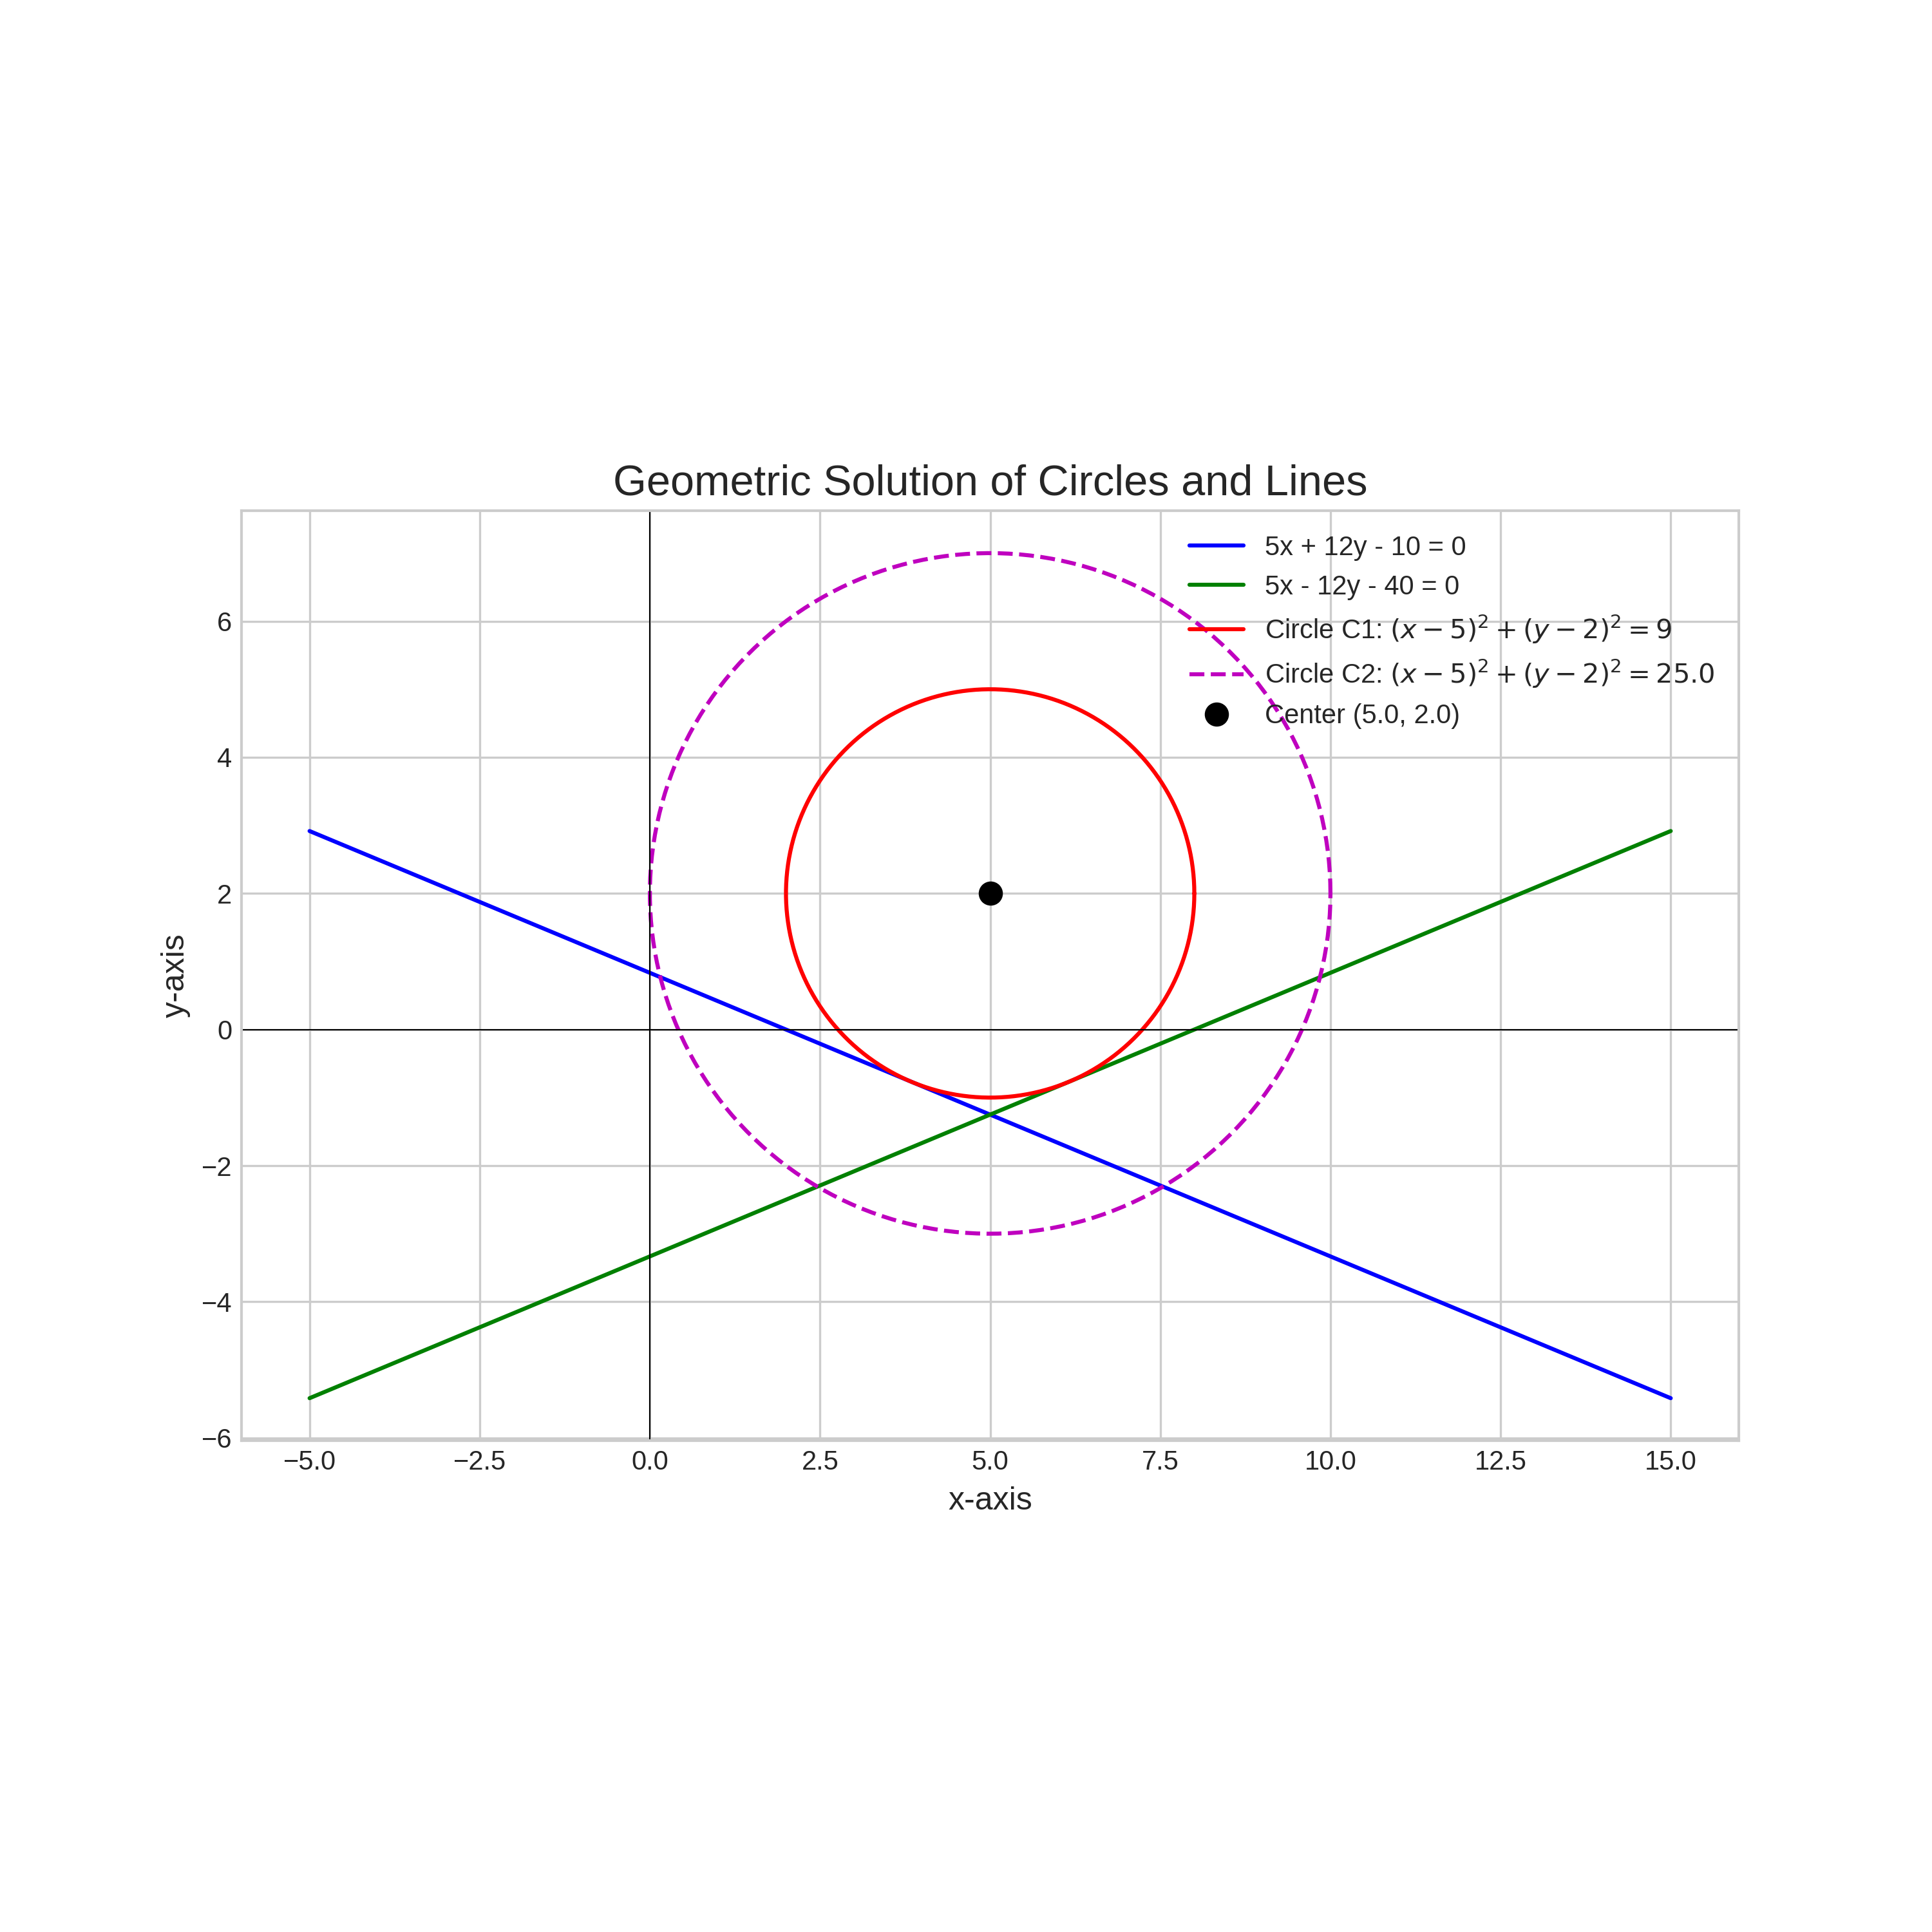
\includegraphics[width=0.8\columnwidth]{figs/figure.png}
        \caption{}
        \label{fig:placeholder}
    \end{figure}
\end{frame}
\begin{frame}[fragile]
\frametitle{Direct Python}
\begin{lstlisting}
import numpy as np
import matplotlib.pyplot as plt

line1_coeffs = np.array([5, 12, -10])
line2_coeffs = np.array([5, -12, -40])


A = np.array([[line1_coeffs[0], line1_coeffs[1]],
              [line2_coeffs[0], line2_coeffs[1]]])
b = np.array([-line1_coeffs[2], -line2_coeffs[2]])


intersection_point = np.linalg.solve(A, b) # Returns [5., -1.25]
h = intersection_point[0]
r1 = 3
k = 2
center = np.array([h, k])
\end{lstlisting}
\end{frame}
\begin{frame}[fragile]
\frametitle{Direct Python}
\begin{lstlisting}

intercept_length = 8
half_intercept = intercept_length / 2.0


r2 = np.hypot(r1, half_intercept) # np.hypot(3, 4) = 5


print("--- Solution (calculated with NumPy) ---")
print(f"Intersection of lines: {intersection_point}")
print(f"Center of circles C1 and C2: ({center[0]}, {center[1]})")
\end{lstlisting}
\end{frame}
\begin{frame}[fragile]
\frametitle{Direct Python}
\begin{lstlisting}
print(f"Radius of circle C1: {r1}")
print(f"Radius of circle C2: {r2}")
print("\nThe equation of circle C2 is:")
print(f"(x - {center[0]})**2 + (y - {center[1]})**2 = {r2**2}")
print("-----------------------------------------")

\end{lstlisting}
\end{frame}
\begin{frame}[fragile]
\frametitle{Direct Python}
\begin{lstlisting}

def get_circle_points(center_h, center_k, radius):
    """Generates x and y coordinates for a circle."""
    theta = np.linspace(0, 2 * np.pi, 200)
    x = center_h + radius * np.cos(theta)
    y = center_k + radius * np.sin(theta)
    return x, y


x_c1, y_c1 = get_circle_points(center[0], center[1], r1)
x_c2, y_c2 = get_circle_points(center[0], center[1], r2)


x_vals = np.linspace(-5, 15, 400)

\end{lstlisting}
\end{frame}
\begin{frame}[fragile]
\frametitle{Direct Python}
\begin{lstlisting}
y_line1 = (-line1_coeffs[0] * x_vals - line1_coeffs[2]) / line1_coeffs[1]

y_line2 = (-line2_coeffs[0] * x_vals - line2_coeffs[2]) / line2_coeffs[1]


plt.style.use('seaborn-v0_8-whitegrid')
fig, ax = plt.subplots(figsize=(10, 10))


ax.plot(x_vals, y_line1, 'b-', label='5x + 12y - 10 = 0')
ax.plot(x_vals, y_line2, 'g-', label='5x - 12y - 40 = 0')
\end{lstlisting}
\end{frame}
\begin{frame}[fragile]
\frametitle{Direct Python}
\begin{lstlisting}

ax.plot(x_c1, y_c1, 'r-', label=f'Circle C1: $(x-5)^2 + (y-2)^2 = {r1**2}$')
ax.plot(x_c2, y_c2, 'm--', label=f'Circle C2: $(x-5)^2 + (y-2)^2 = {r2**2}$')

ax.plot(center[0], center[1], 'ko', markersize=8, label=f'Center ({center[0]}, {center[1]})')


ax.set_title('Geometric Solution of Circles and Lines', fontsize=16)
ax.set_xlabel('x-axis', fontsize=12)
ax.set_ylabel('y-axis', fontsize=12)
ax.legend(fontsize=10)
\end{lstlisting}
\end{frame}
\begin{frame}[fragile]
\frametitle{Direct Python}
\begin{lstlisting}
ax.axhline(0, color='black', linewidth=0.5)
ax.axvline(0, color='black', linewidth=0.5)

ax.set_aspect('equal', adjustable='box')
plt.savefig("figure.png", dpi=300)
plt.show()
\end{lstlisting}
\end{frame}
\begin{frame}[fragile]
\frametitle{C code}
\begin{lstlisting}
#include <stdio.h>
#include <math.h>

struct Circle {
    double h, k, r;
};
struct Circle find_C1() {
    struct Circle c1;
    c1.h = 5.0;
    c1.k = 2.0;
    c1.r = 3.0;
    return c1;
}
struct Circle find_C2(struct Circle c1, double L) {
    struct Circle c2;
    \end{lstlisting}
\end{frame}
\begin{frame}[fragile]
\frametitle{C code}
\begin{lstlisting}
    c2.h = c1.h;
    c2.k = c1.k;
  
    double d = 3.0;
    c2.r = sqrt(pow(L/2, 2) + pow(d, 2));
    return c2;
}
void get_circles(double *h1, double *k1, double *r1, double *h2, double *k2, double *r2) {
    struct Circle c1 = find_C1();
    struct Circle c2 = find_C2(c1, 8.0);

    *h1 = c1.h; *k1 = c1.k; *r1 = c1.r;
    *h2 = c2.h; *k2 = c2.k; *r2 = c2.r;
}
\end{lstlisting}
\end{frame}
\begin{frame}[fragile]
\frametitle{Python code with shared object}
\begin{lstlisting}
import ctypes
import numpy as np
import matplotlib.pyplot as plt


lib = ctypes.CDLL('./main.so')


lib.get_circles.argtypes = [
    ctypes.POINTER(ctypes.c_double), ctypes.POINTER(ctypes.c_double), ctypes.POINTER(ctypes.c_double),
    ctypes.POINTER(ctypes.c_double), ctypes.POINTER(ctypes.c_double), ctypes.POINTER(ctypes.c_double)
]
\end{lstlisting}
\end{frame}
\begin{frame}[fragile]
\frametitle{Python code with shared object}
\begin{lstlisting}

h1 = ctypes.c_double()
k1 = ctypes.c_double()
r1 = ctypes.c_double()
h2 = ctypes.c_double()
k2 = ctypes.c_double()
r2 = ctypes.c_double()

# Call C function
lib.get_circles(ctypes.byref(h1), ctypes.byref(k1), ctypes.byref(k2), ctypes.byref(h2), ctypes.byref(k2), ctypes.byref(r2))
\end{lstlisting}
\end{frame}
\begin{frame}[fragile]
\frametitle{Python code with shared object}
\begin{lstlisting}
# But fix: k2 got used twice → fix proper call
lib.get_circles(ctypes.byref(h1), ctypes.byref(k1), ctypes.byref(r1), ctypes.byref(h2), ctypes.byref(k2), ctypes.byref(r2))

# Extract values
h1, k1, r1 = h1.value, k1.value, r1.value
h2, k2, r2 = h2.value, k2.value, r2.value
\end{lstlisting}
\end{frame}
\begin{frame}[fragile]
\frametitle{Python code with shared object}
\begin{lstlisting}
# Plot circles and lines
theta = np.linspace(0, 2*np.pi, 400)
x1, y1 = h1 + r1*np.cos(theta), k1 + r1*np.sin(theta)
x2, y2 = h2 + r2*np.cos(theta), k2 + r2*np.sin(theta)

plt.figure(figsize=(7,7))
plt.plot(x1, y1, 'b', label='Circle C1')
plt.plot(x2, y2, 'g', label='Circle C2')
\end{lstlisting}
\end{frame}
\begin{frame}[fragile]
\frametitle{Python code with shared object}
\begin{lstlisting}
# Plot lines
x = np.linspace(-5, 15, 400)
y_line1 = (-5*x + 10)/12
y_line2 = (5*x - 40)/12
plt.plot(x, y_line1, 'r--', label='Line 1')
plt.plot(x, y_line2, 'r-.', label='Line 2')
\end{lstlisting}
\end{frame}
\begin{frame}[fragile]
\frametitle{Python code with shared object}
\begin{lstlisting}
# Format plot
plt.gca().set_aspect('equal', adjustable='box')
plt.grid(True)
plt.legend()
plt.title('Circles C1 & C2 with Tangent Lines')
plt.xlabel('x')
plt.ylabel('y')
plt.show()
\end{lstlisting}
\end{frame}

\end{document}